\documentclass[conference]{IEEEtran}
\usepackage[T1]{fontenc}
\usepackage{cite}
\usepackage{amsmath}
\usepackage{booktabs}
\usepackage{url}
\usepackage{tikz}
\usetikzlibrary{positioning,arrows.meta,fit}
\usepackage[hidelinks]{hyperref}

\begin{document}

\title{A Holarchy of Coding Agents:\\
An Industrial Experience Report on a Koestler-Inspired\\
Multi-Agent System for Ticket-to-Pull-Request Automation}

\author{\IEEEauthorblockN{Luis Felipe Soares Coelho}
\IEEEauthorblockA{Independent Researcher, Brazil\\
felipecoelho.ness@gmail.com}}

\maketitle

\begin{abstract}
Autonomous coding agents are moving from single sessions toward systems of
agents that react to tickets and events and return pull requests (PRs). A
recurring architectural answer is a flat \emph{router/worker} split, recently
proposed again by DeepSeek's ``super-agent'' design. We report on an
alternative built and deployed at a Brazilian B2B SaaS company between March
and August 2026: a multi-agent system designed as a \emph{holarchy} in the
sense of Koestler, where each agent (\emph{holon}) is at once an autonomous
whole and a cooperative part. The system takes an issue-tracker ticket,
localises code through a seven-layer search, runs fifteen parallel LLM
runners with distinct repair strategies, ranks them with deterministic
scores, and opens a PR. We describe two generations of the system, a code
audit that compares the intended holarchy with what the code actually does,
and field data: 22 PRs on 11 tickets in 6 repositories, opened by 4
engineers, of which 2 PRs (one ticket) were merged; plus 17 autonomous
investigation PRs and 9 ticket analyses. The holonic properties realised
in production are delegated authority over an irreversible action, an
upward channel through which runner behaviour revises the parent's
diagnosis, and autonomous origination of work; an explicit negotiation
protocol between holons was designed but remains unwired. We distil five
lessons, chiefly that correctness proxies, repository selection
and PR hygiene dominated outcomes far more than agent topology.
\end{abstract}

\begin{IEEEkeywords}
LLM agents, multi-agent systems, holonic systems, automated program repair, experience report
\end{IEEEkeywords}

\section{Introduction}

LLM-based agents now resolve a meaningful share of benchmark issues
\cite{jimenez2024swebench,yang2024sweagent,wang2025openhands,xia2024agentless},
and practitioners are composing them into systems that act on real
engineering workflows. The bottleneck is shifting from the model to
human attention: a developer can supervise only a handful of agent sessions
at once \cite{deepseek2026superagent}. Architectures that let agents take
work from tickets and events without per-task prompting are therefore
attractive.

Most such architectures are command hierarchies: authority sits at the top
and parts only execute. DeepSeek's super-agent prototype
\cite{deepseek2026superagent} is representative: a router session receives
triggers, evaluates them, and launches one executor session per ticket;
executors report to the router and have no tool to message one another.
Role-play frameworks such as MetaGPT \cite{hong2024metagpt} and ChatDev
\cite{qian2024chatdev} also fix the chain of command.

Manufacturing faced a similar tension three decades ago and answered with
\emph{holonic} systems \cite{vanbrussel1998prosa,gerber1999holonic,giret2004holons},
built on Koestler's notion of the holon \cite{koestler1967}: a unit that is
self-assertive toward its parts and integrative toward its whole (the
``Janus effect''). A holarchy is a nesting of such units. It has levels,
but it is not a command hierarchy: each holon governs itself by its own
rules, decides within its scope without asking the level above, and
informs that level in return. Authority is distributed along the levels
rather than concentrated at the top.

This paper reports on applying that idea to ticket-to-PR automation.
The author designed and built the system as an individual engineer.
It was first prototyped publicly in March 2026
\cite{coelho2026book,coelho2026prototypes}, evolved through two generations,
and was used on production repositories. Our contributions are:
\begin{itemize}
  \item a holarchic architecture for coding agents and its mapping onto a
        concrete pipeline (Section~\ref{sec:design});
  \item a code-level audit that separates what was implemented from what was
        only designed, an analysis rarely reported for agent systems
        (Section~\ref{sec:audit});
  \item field data from real use, including failures
        (Section~\ref{sec:field}); and
  \item lessons for practitioners, contrasted with the router/worker
        alternative (Section~\ref{sec:lessons}).
\end{itemize}

\section{Background and Related Work}
\label{sec:related}

\textbf{Holonic systems.} PROSA \cite{vanbrussel1998prosa} defined product,
resource and order holons for manufacturing control; holonic multi-agent
systems \cite{gerber1999holonic,giret2004holons} generalised the idea to
software agents that can merge into super-holons and negotiate. The closest
recent work is Ashfaq et~al.\ \cite{ashfaq2025holonic}, which proposes LLM
reasoning inside supervisor, planner and task holons for systems of systems.
That proposal is conceptual and targets smart-city mobility. To our
knowledge no prior report describes an implemented, field-used holarchic
architecture for software engineering.

\textbf{LLM agents for software engineering.} Single-agent systems
\cite{yang2024sweagent,wang2025openhands,zhang2024autocoderover} and fixed
pipelines \cite{xia2024agentless} dominate issue resolution. Multi-agent
frameworks \cite{hong2024metagpt,qian2024chatdev,wu2023autogen} coordinate
roles through conversation; surveys catalogue the space
\cite{he2024lmasurvey,liu2024agentsurvey}. Our runner layer is closest to
repeated sampling with a verifier \cite{brown2024monkeys,chen2023codet}, but
with heterogeneous strategies and a feedback edge into diagnosis.

\section{Design: A Holarchy for Ticket-to-PR}
\label{sec:design}

\begin{figure}[t]
\centering
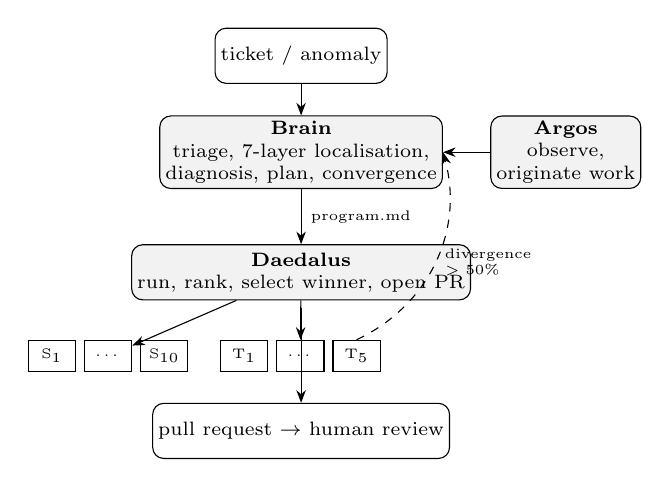
\begin{tikzpicture}[
  node distance=4mm and 3mm,
  holon/.style={draw,rounded corners,align=center,font=\scriptsize,minimum height=7mm,inner sep=2pt},
  run/.style={draw,align=center,font=\tiny,minimum width=6mm,minimum height=4mm,inner sep=1pt},
  arr/.style={-{Stealth[length=1.6mm]}},
  up/.style={-{Stealth[length=1.6mm]},dashed}
]
\node[holon,fill=gray!10] (brain) {\textbf{Brain}\\triage, 7-layer localisation,\\diagnosis, plan, convergence};
\node[holon,fill=gray!10,below=7mm of brain] (daed) {\textbf{Daedalus}\\run, rank, select winner, open PR};
\node[run,below left=5mm and 7mm of daed] (s1) {S\textsubscript{1}};
\node[run,right=1mm of s1] (s2) {\dots};
\node[run,right=1mm of s2] (s10) {S\textsubscript{10}};
\node[run,right=4mm of s10] (t1) {T\textsubscript{1}};
\node[run,right=1mm of t1] (t2) {\dots};
\node[run,right=1mm of t2] (t5) {T\textsubscript{5}};
\node[holon,right=6mm of brain,fill=gray!10] (argos) {\textbf{Argos}\\observe,\\originate work};
\node[holon,above=4mm of brain] (tix) {ticket / anomaly};
\node[holon,below=13mm of daed] (pr) {pull request $\rightarrow$ human review};
\draw[arr] (tix) -- (brain);
\draw[arr] (brain) -- node[right,font=\tiny]{program.md} (daed);
\draw[arr] (daed) -- (s2);
\draw[arr] (daed) -- (t2);
\draw[up] (t5.north) to[bend right=40] node[right,font=\tiny,align=left]{divergence\\$>50\%$} (brain.east);
\draw[arr] (daed.south) ++(0,-0.1) -- (pr);
\draw[arr] (argos) -- (brain);
\end{tikzpicture}
\caption{The holarchy as deployed. Solid arrows: delegation. Dashed arrow:
the upward channel by which thinker runners revise Brain's diagnosis.
S: snipers, T: thinkers.}
\label{fig:arch}
\end{figure}

\textbf{Holons.} The system has three holons (Fig.~\ref{fig:arch}).
\emph{Brain} owns understanding: it watches the tracker, triages the ticket
(bug, false positive, needs information), selects the repository, localises
code, diagnoses a root cause and writes a plan. \emph{Daedalus} owns change:
it turns the plan into competing patches and decides which one ships.
\emph{Argos} owns observation: it polls monitoring and tracker sources and can
originate work. Each holon is a separate process with its own API and store.
The design intent, stated in the system's documentation, was that holons
``propose, evaluate and decide together''.

\textbf{Localisation.} Brain extracts search terms from the ticket in two
languages and several identifier styles, then runs seven layers:
exact \texttt{git grep}, cross-term regex, path filtering, an LLM pass over
the tree, recently modified files, test-to-source inference, and an LLM pass
over entry points. The two LLM layers run only when fewer than three files
have been found. Files are ranked by how many layers hit them.

\textbf{Competing runners.} Daedalus runs ten \emph{sniper} runners in git
worktrees, each with a narrow strategy (inline fix, guard, validation,
condition fix, fallback, import, async, extraction, type check,
simplification). It also runs five \emph{thinker} runners in separate
processes with broader strategies (fix with tests, module refactor,
architectural fix, comprehensive fix, defensive rewrite) and a larger
context window (25k vs.\ 12k characters). Each runner scores itself with a
deterministic rubric worth 100 points: tests passing, diff size, absence of
unsafe type casts, no new dependencies, import hygiene, touching a target
file, and lint-like checks. The final rank is
$0.5\,s_{\mathrm{self}} + 0.3\min(5\,n_{\mathrm{pass}},100) + 20\,[\Delta > 0]$.

\textbf{Upward correction.} After each round, Brain compares the files the
thinker runners edited with its own predicted file set. If more than half
fall outside the prediction, Brain treats its hypothesis as falsified,
merges both views into a revised diagnosis and re-delegates, for at most
three rounds. A subordinate's behaviour thus changes the superordinate's
belief, which is the integrative face of the holon made operational.

\textbf{Delegated authority.} Daedalus, not Brain, selects the winner, pushes
the branch and opens the PR. Brain's later LLM validation annotates the
result but cannot retract it. The part holds authority over an irreversible
action, which a pure worker does not.

\textbf{Second generation.} \emph{Nous} (May--August 2026) placed a
conversational meta-holon above Brain and moved Argos to the front of an
autonomous chain: a monitoring scout detects a slow endpoint, Nous opens a
ticket, Brain writes an investigation PR, and optionally a fix is drafted
and debated by five LLM personas before a human decides. Nous can veto a
Brain plan that violates the user's stated hard preferences, and request
one reformulation.

\textbf{Implementation.} The first generation comprises 287 commits (20 Mar
to 7 Apr 2026) in TypeScript with an append-only Postgres event store and a
CQRS projection for graph memory; the second has 353 commits and about 46k
lines of TypeScript plus a small Python service. The three public prototypes
\cite{coelho2026prototypes} carry 970 passing tests at the time of writing.
All runners used one mid-tier commercial model (Claude Sonnet 4).

\section{Design Versus Code: An Audit}
\label{sec:audit}

Agent papers usually describe intended architectures. We audited both
generations against their source in November 2026, labelling each claim as
implemented-and-tested, implemented, or design-only. Table~\ref{tab:audit}
summarises the holarchic properties.

\begin{table}[t]
\caption{Holarchic properties, intended vs.\ reachable in code (impl.: implemented; +T: covered by tests)}
\label{tab:audit}
\centering
\footnotesize
\setlength{\tabcolsep}{3pt}
\begin{tabular}{@{}p{3.3cm}p{1.25cm}p{3.6cm}@{}}
\toprule
Property & Status & Evidence \\
\midrule
Delegated irreversible action (winner, PR) & impl. & Daedalus opens PR before Brain validates \\
Upward revision of parent belief & impl.+T & divergence $>0.5$, $\le$3 rounds \\
Autonomous origination of work & impl. & Argos scout $\rightarrow$ intake (gen.\,2) \\
Parent veto with reformulation & impl.+T & 1 counter round (gen.\,2) \\
Subordinate refusal / counter-proposal & design & statuses declared, never produced \\
Peer messaging between runners & absent & runners isolated by design \\
Asynchronous holon integration & absent & blocking HTTP, up to 15\,min \\
\bottomrule
\end{tabular}
\end{table}

Three findings matter beyond this system. First, \emph{the holarchy held,
but its negotiation layer was left unwired under delivery pressure}: each
holon kept its own scope of decision, yet the sequence between them became a
fixed script, while the richer agent loop (a 15-state machine and 29 tools)
was never wired to the server. Negotiation endpoints exist but always
accept. Second, \emph{documentation overstated the code}: the
documented scoring rubric is dead code, the ``thinkers'' were described as a
stronger model but ran the same one, and the state count differed. Third,
\emph{contracts drifted between holons}: in the second generation the chat
path's delegation payload no longer matched Daedalus's schema and was
rejected with HTTP~400; cost and time cut-offs existed but were disabled on
the main loop. Seven corrective commits were needed in November 2026 to
restore the multi-runner path. Independent processes with separate
contracts make such drift easy and silent; contract tests between holons
would have caught it.

\section{Field Use}
\label{sec:field}

\textbf{Method.} The PR body generated by Daedalus contains a distinctive
section (a per-runner analysis table). We searched the company's GitHub
organisation for it, then read state, target branch and closing comments of
every hit. We did the same for the ticket-analysis comment, the
investigation-PR branch prefix and the debate marker of the second
generation. The company and its repositories are anonymised.

\begin{table}[t]
\caption{Field data, March--May 2026}
\label{tab:field}
\centering
\footnotesize
\begin{tabular}{@{}lr@{}}
\toprule
\multicolumn{2}{@{}l}{\emph{Generation 1: ticket-to-PR}} \\
PRs opened & 22 \\
\quad distinct tickets (incl.\ 1 test run) & 11 \\
\quad repositories & 6 \\
\quad engineers who ran it (PR authors) & 4 \\
\quad by month (Mar / Apr / May) & 16 / 1 / 5 \\
PRs merged & 2 (1 ticket, 2 branches) \\
PRs closed without merge & 19 \\
PRs still open & 1 \\
Tickets with an automated analysis comment & 9 \\
\midrule
\multicolumn{2}{@{}l}{\emph{Generation 2: monitoring-to-investigation}} \\
Investigation PRs (one day) & 17, none merged \\
PRs with a five-persona debate verdict & 3 \\
\midrule
\multicolumn{2}{@{}l}{\emph{Early live test (4 tickets, 20 Mar)}} \\
Triage / localisation succeeded & 4/4, 4/4 \\
PRs produced & 0/4 (edit-format parsing) \\
Mean wall time per ticket & 36.4\,s \\
\bottomrule
\end{tabular}
\end{table}

\textbf{Adoption.} Table~\ref{tab:field} shows that three engineers other
than the author ran the system on their own tickets (9 of the 22 PRs), in
March and again in May, without any mandate to do so. Two engineers
reported also using the system's review mode to draft code-review comments.
We could not verify this from artefacts: that mode deliberately produces
plain prose without markers, and the two engineers' 717 inline review
comments in the period carry no machine fingerprint. We therefore treat it
as self-reported.

\textbf{Outcomes.} One of ten real tickets reached production through the
system's own PRs, merged on both the release and development branches after
about ten days.
Closing comments on the other PRs reveal the failure modes:
\begin{itemize}
  \item \emph{Duplicate PRs per ticket.} Each convergence round that found a
        winner opened its own PR; one ticket accumulated six PRs and another
        three. Many of the 19 closures are such duplicates or later
        backlog clean-ups after two months without activity.
  \item \emph{Wrong repository.} One ticket was localised in a sibling
        repository and patched there.
  \item \emph{Stale base.} One PR was cut from an outdated branch and carried
        103 unrelated files.
  \item \emph{Misdiagnosis.} In the second generation, all 17 investigation
        PRs were closed; the one we examined in depth blamed a Markdown
        documentation file because the endpoint's code lived in another
        repository.
\end{itemize}
No closing comment cited a defect in the generated code itself. The
evidence is too thin to claim code quality, but it does show where the
system lost: before and after code generation, not inside it.

\textbf{Cost.} The only fully instrumented run (a synthetic ticket through
the agent loop) consumed 481k input and 14k output tokens over 20 turns,
about US\$2.76. The deterministic pipeline used in the field is cheaper per
call but runs fifteen runners per round.

\section{Lessons}
\label{sec:lessons}

\textbf{L1: Start from the holonic properties that cost little.} Delegated
authority and upward correction were cheap to build and held through every
refactoring. An explicit negotiation protocol was expensive and was
deferred. A holarchy of agents can start from autonomy and upward
correction and add negotiation once those are stable.

\textbf{L2: Topology mattered less than the edges of the pipeline.}
Repository selection, base-branch freshness and PR deduplication caused most
losses. Router/worker designs \cite{deepseek2026superagent} face the same
edges; the holarchy did not remove them.

\textbf{L3: Deterministic scores are not correctness.} Our rubric rewarded
small, typed, dependency-free diffs, and, in repositories without tests,
ranking fell back to size and style alone. Repeated sampling only pays when
the verifier measures the property of interest
\cite{brown2024monkeys,chen2023codet}.

\textbf{L4: Audit the design you publish.} Every overstatement we found
(model, rubric, states, negotiation) was in documentation written during a
competition deadline. A reachability audit took less time than writing the
original documentation.

\textbf{L5: Measure adoption, not only accuracy.} A 1-in-10 merge rate looks
poor, yet engineers kept choosing to run the system. Field reports should
record who used an agent and for what, alongside whether its PRs were
merged.

\textbf{Threats to validity.} The data come from one company, two
generations and a small number of tickets. Fingerprint search finds only
artefacts that kept the generated text; PRs that engineers rewrote by hand
are invisible, so the merge rate is a lower bound on influence. The author
built the system and conducted the audit.

\section{Conclusion}

A Koestler-style holarchy is a useful lens for agent systems: it names the
two properties (authority delegated to parts, information flowing up to
revise the whole) that distinguish a holon from a worker. Our deployment
realised both in production; negotiation between holons is the part still
to be built.
DeepSeek's recent super-agent \cite{deepseek2026superagent} keeps the router
in charge of every decision; our experience suggests that letting the part
decide, and letting it correct the whole, is feasible in production today.
Our next step is a controlled evaluation on resolved tickets with known
human fixes, using the repaired multi-runner path.

\bibliographystyle{IEEEtran}
\bibliography{refs}

\end{document}
